\PassOptionsToPackage{unicode=true}{hyperref} % options for packages loaded elsewhere
\PassOptionsToPackage{hyphens}{url}
%
\documentclass[]{article}
\usepackage{lmodern}
\usepackage{amssymb,amsmath}
\usepackage{ifxetex,ifluatex}
\usepackage{fixltx2e} % provides \textsubscript
\ifnum 0\ifxetex 1\fi\ifluatex 1\fi=0 % if pdftex
  \usepackage[T1]{fontenc}
  \usepackage[utf8]{inputenc}
  \usepackage{textcomp} % provides euro and other symbols
\else % if luatex or xelatex
  \usepackage{unicode-math}
  \defaultfontfeatures{Ligatures=TeX,Scale=MatchLowercase}
\fi
% use upquote if available, for straight quotes in verbatim environments
\IfFileExists{upquote.sty}{\usepackage{upquote}}{}
% use microtype if available
\IfFileExists{microtype.sty}{%
\usepackage[]{microtype}
\UseMicrotypeSet[protrusion]{basicmath} % disable protrusion for tt fonts
}{}
\IfFileExists{parskip.sty}{%
\usepackage{parskip}
}{% else
\setlength{\parindent}{0pt}
\setlength{\parskip}{6pt plus 2pt minus 1pt}
}
\usepackage{hyperref}
\hypersetup{
            pdftitle={Covid 19 en México},
            pdfauthor={Murpholinox Peligro},
            pdfborder={0 0 0},
            breaklinks=true}
\urlstyle{same}  % don't use monospace font for urls
\usepackage[margin=1in]{geometry}
\usepackage{color}
\usepackage{fancyvrb}
\newcommand{\VerbBar}{|}
\newcommand{\VERB}{\Verb[commandchars=\\\{\}]}
\DefineVerbatimEnvironment{Highlighting}{Verbatim}{commandchars=\\\{\}}
% Add ',fontsize=\small' for more characters per line
\usepackage{framed}
\definecolor{shadecolor}{RGB}{248,248,248}
\newenvironment{Shaded}{\begin{snugshade}}{\end{snugshade}}
\newcommand{\AlertTok}[1]{\textcolor[rgb]{0.94,0.16,0.16}{#1}}
\newcommand{\AnnotationTok}[1]{\textcolor[rgb]{0.56,0.35,0.01}{\textbf{\textit{#1}}}}
\newcommand{\AttributeTok}[1]{\textcolor[rgb]{0.77,0.63,0.00}{#1}}
\newcommand{\BaseNTok}[1]{\textcolor[rgb]{0.00,0.00,0.81}{#1}}
\newcommand{\BuiltInTok}[1]{#1}
\newcommand{\CharTok}[1]{\textcolor[rgb]{0.31,0.60,0.02}{#1}}
\newcommand{\CommentTok}[1]{\textcolor[rgb]{0.56,0.35,0.01}{\textit{#1}}}
\newcommand{\CommentVarTok}[1]{\textcolor[rgb]{0.56,0.35,0.01}{\textbf{\textit{#1}}}}
\newcommand{\ConstantTok}[1]{\textcolor[rgb]{0.00,0.00,0.00}{#1}}
\newcommand{\ControlFlowTok}[1]{\textcolor[rgb]{0.13,0.29,0.53}{\textbf{#1}}}
\newcommand{\DataTypeTok}[1]{\textcolor[rgb]{0.13,0.29,0.53}{#1}}
\newcommand{\DecValTok}[1]{\textcolor[rgb]{0.00,0.00,0.81}{#1}}
\newcommand{\DocumentationTok}[1]{\textcolor[rgb]{0.56,0.35,0.01}{\textbf{\textit{#1}}}}
\newcommand{\ErrorTok}[1]{\textcolor[rgb]{0.64,0.00,0.00}{\textbf{#1}}}
\newcommand{\ExtensionTok}[1]{#1}
\newcommand{\FloatTok}[1]{\textcolor[rgb]{0.00,0.00,0.81}{#1}}
\newcommand{\FunctionTok}[1]{\textcolor[rgb]{0.00,0.00,0.00}{#1}}
\newcommand{\ImportTok}[1]{#1}
\newcommand{\InformationTok}[1]{\textcolor[rgb]{0.56,0.35,0.01}{\textbf{\textit{#1}}}}
\newcommand{\KeywordTok}[1]{\textcolor[rgb]{0.13,0.29,0.53}{\textbf{#1}}}
\newcommand{\NormalTok}[1]{#1}
\newcommand{\OperatorTok}[1]{\textcolor[rgb]{0.81,0.36,0.00}{\textbf{#1}}}
\newcommand{\OtherTok}[1]{\textcolor[rgb]{0.56,0.35,0.01}{#1}}
\newcommand{\PreprocessorTok}[1]{\textcolor[rgb]{0.56,0.35,0.01}{\textit{#1}}}
\newcommand{\RegionMarkerTok}[1]{#1}
\newcommand{\SpecialCharTok}[1]{\textcolor[rgb]{0.00,0.00,0.00}{#1}}
\newcommand{\SpecialStringTok}[1]{\textcolor[rgb]{0.31,0.60,0.02}{#1}}
\newcommand{\StringTok}[1]{\textcolor[rgb]{0.31,0.60,0.02}{#1}}
\newcommand{\VariableTok}[1]{\textcolor[rgb]{0.00,0.00,0.00}{#1}}
\newcommand{\VerbatimStringTok}[1]{\textcolor[rgb]{0.31,0.60,0.02}{#1}}
\newcommand{\WarningTok}[1]{\textcolor[rgb]{0.56,0.35,0.01}{\textbf{\textit{#1}}}}
\usepackage{graphicx,grffile}
\makeatletter
\def\maxwidth{\ifdim\Gin@nat@width>\linewidth\linewidth\else\Gin@nat@width\fi}
\def\maxheight{\ifdim\Gin@nat@height>\textheight\textheight\else\Gin@nat@height\fi}
\makeatother
% Scale images if necessary, so that they will not overflow the page
% margins by default, and it is still possible to overwrite the defaults
% using explicit options in \includegraphics[width, height, ...]{}
\setkeys{Gin}{width=\maxwidth,height=\maxheight,keepaspectratio}
\setlength{\emergencystretch}{3em}  % prevent overfull lines
\providecommand{\tightlist}{%
  \setlength{\itemsep}{0pt}\setlength{\parskip}{0pt}}
\setcounter{secnumdepth}{0}
% Redefines (sub)paragraphs to behave more like sections
\ifx\paragraph\undefined\else
\let\oldparagraph\paragraph
\renewcommand{\paragraph}[1]{\oldparagraph{#1}\mbox{}}
\fi
\ifx\subparagraph\undefined\else
\let\oldsubparagraph\subparagraph
\renewcommand{\subparagraph}[1]{\oldsubparagraph{#1}\mbox{}}
\fi

% set default figure placement to htbp
\makeatletter
\def\fps@figure{htbp}
\makeatother


\title{Covid 19 en México}
\author{Murpholinox Peligro}
\date{19 de abril del 2020}

\begin{document}
\maketitle

\begin{Shaded}
\begin{Highlighting}[]
\CommentTok{# Carga los paquetes necesarios.}
\KeywordTok{library}\NormalTok{(ggplot2)}
\KeywordTok{library}\NormalTok{(ggdark)}
\KeywordTok{library}\NormalTok{(latex2exp)}
\KeywordTok{library}\NormalTok{(lubridate)}
\KeywordTok{library}\NormalTok{(dplyr)}
\CommentTok{# Configura el directorio de trabajo.}
\KeywordTok{setwd}\NormalTok{(}\StringTok{"/home/murphy/Repos/plotcovid19mx"}\NormalTok{)}
\end{Highlighting}
\end{Shaded}

\begin{Shaded}
\begin{Highlighting}[]
\CommentTok{# Descarga datos del European CDC.}
\FunctionTok{wget}\NormalTok{ -O full.csv https://opendata.ecdc.europa.eu/covid19/casedistribution/csv}
\CommentTok{# Obtiene las líneas correspondientes a México.}
\FunctionTok{grep}\NormalTok{ Mex full.csv }\OperatorTok{>}\NormalTok{ mex.csv}
\CommentTok{# Solo ocupamos la columna 1 y 6 (fecha y decesos por día).}
\FunctionTok{awk}\NormalTok{ -F }\StringTok{","} \StringTok{'\{print $1"," $6\}'}\NormalTok{ mex.csv }\OperatorTok{>}\NormalTok{ clean.csv}
\CommentTok{# Añade nombre a las columnas.}
\BuiltInTok{echo} \StringTok{"fecha,decesos"} \OperatorTok{>>}\NormalTok{ clean.csv}
\CommentTok{# Revierte los datos en la lista.}
\FunctionTok{tac}\NormalTok{ clean.csv }\OperatorTok{>}\NormalTok{ clean_r.csv}
\end{Highlighting}
\end{Shaded}

\begin{verbatim}
## --2020-04-22 19:06:45--  https://opendata.ecdc.europa.eu/covid19/casedistribution/csv
## Resolving opendata.ecdc.europa.eu (opendata.ecdc.europa.eu)... 212.181.0.63
## Connecting to opendata.ecdc.europa.eu (opendata.ecdc.europa.eu)|212.181.0.63|:443... connected.
## HTTP request sent, awaiting response... 301 Moved Permanently
## Location: https://opendata.ecdc.europa.eu/covid19/casedistribution/csv/ [following]
## --2020-04-22 19:06:46--  https://opendata.ecdc.europa.eu/covid19/casedistribution/csv/
## Reusing existing connection to opendata.ecdc.europa.eu:443.
## HTTP request sent, awaiting response... 200 OK
## Length: 720081 (703K) [application/octet-stream]
## Saving to: ‘full.csv’
## 
##      0K .......... .......... .......... .......... ..........  7%  222K 3s
##     50K .......... .......... .......... .......... .......... 14%  229K 3s
##    100K .......... .......... .......... .......... .......... 21%  231K 2s
##    150K .......... .......... .......... .......... .......... 28%  241K 2s
##    200K .......... .......... .......... .......... .......... 35%  246K 2s
##    250K .......... .......... .......... .......... .......... 42% 2.12M 1s
##    300K .......... .......... .......... .......... .......... 49%  234K 1s
##    350K .......... .......... .......... .......... .......... 56%  245K 1s
##    400K .......... .......... .......... .......... .......... 63%  234K 1s
##    450K .......... .......... .......... .......... .......... 71%  242K 1s
##    500K .......... .......... .......... .......... .......... 78% 2.35M 1s
##    550K .......... .......... .......... .......... .......... 85%  238K 0s
##    600K .......... .......... .......... .......... .......... 92%  109K 0s
##    650K .......... .......... .......... .......... .......... 99% 32.5K 0s
##    700K ...                                                   100% 6111G=4.2s
## 
## 2020-04-22 19:06:51 (169 KB/s) - ‘full.csv’ saved [720081/720081]
\end{verbatim}

\begin{Shaded}
\begin{Highlighting}[]
\CommentTok{# Carga los datos limpios a R.}
\NormalTok{datos <-}\StringTok{ }\KeywordTok{read.csv}\NormalTok{(}\StringTok{"~/Repos/plotcovid19mx/clean_r.csv"}\NormalTok{)}
\CommentTok{# Cambia el formato de la fecha de d/m/y a y-m-d.}
\NormalTok{datos}\OperatorTok{$}\NormalTok{newdate <-}\StringTok{ }\NormalTok{lubridate}\OperatorTok{::}\KeywordTok{dmy}\NormalTok{(datos}\OperatorTok{$}\NormalTok{fecha)}
\end{Highlighting}
\end{Shaded}

\begin{Shaded}
\begin{Highlighting}[]
\CommentTok{# Crea una nueva variable con un nuevo formato para la fecha (a números enteros).}
\CommentTok{# Esto se hace porque x con formato de fecha impide que el algoritmo para }
\CommentTok{# obtener el modelo exponencial llegue a una solución.}
\NormalTok{xmax <-}\StringTok{ }\KeywordTok{max}\NormalTok{(}\KeywordTok{length}\NormalTok{(datos}\OperatorTok{$}\NormalTok{fecha))}
\NormalTok{datos}\OperatorTok{$}\NormalTok{number <-}\StringTok{ }\KeywordTok{seq}\NormalTok{(}\DecValTok{0}\NormalTok{,xmax}\DecValTok{-1}\NormalTok{)}
\CommentTok{# Necesitamos los días del brote en México (después del 20-marzo).}
\NormalTok{smalldf<-datos }\OperatorTok
\StringTok{  }\KeywordTok{filter}\NormalTok{(number }\OperatorTok{>=}\StringTok{ }\DecValTok{72}\NormalTok{) }
\CommentTok{# Ordena los datos a usar en un tibble.}
\NormalTok{x<-smalldf}\OperatorTok{$}\NormalTok{number}
\NormalTok{x<-x}\DecValTok{-71}
\NormalTok{y<-smalldf}\OperatorTok{$}\NormalTok{decesos}
\NormalTok{nice<-}\KeywordTok{tibble}\NormalTok{(x,y)}
\CommentTok{# Guarda datos finales en formato CSV.}
\KeywordTok{write.csv}\NormalTok{(nice, }\DataTypeTok{file=}\StringTok{"~/Repos/plotcovid19mx/nice.csv"}\NormalTok{)}
\CommentTok{# Crea una gráfica base.}
\NormalTok{p <-}\StringTok{ }\KeywordTok{ggplot}\NormalTok{(}\DataTypeTok{data =}\NormalTok{ nice, }\KeywordTok{aes}\NormalTok{(}\DataTypeTok{x=}\NormalTok{x, }\DataTypeTok{y=}\NormalTok{y)) }\OperatorTok{+}\StringTok{ }\KeywordTok{geom_point}\NormalTok{()}
\end{Highlighting}
\end{Shaded}

\begin{Shaded}
\begin{Highlighting}[]
\CommentTok{# Crea el modelo exponencial.}
\NormalTok{m <-}\KeywordTok{nls}\NormalTok{(y}\OperatorTok{~}\NormalTok{a}\OperatorTok{*}\KeywordTok{exp}\NormalTok{(b}\OperatorTok{*}\NormalTok{x), }\DataTypeTok{start =} \KeywordTok{list}\NormalTok{(}\DataTypeTok{a=}\FloatTok{0.6}\NormalTok{, }\DataTypeTok{b=}\FloatTok{0.16}\NormalTok{))}
\CommentTok{# Imprime información del modelo.}
\KeywordTok{summary}\NormalTok{(m)}
\end{Highlighting}
\end{Shaded}

\begin{verbatim}
## 
## Formula: y ~ a * exp(b * x)
## 
## Parameters:
##   Estimate Std. Error t value Pr(>|t|)    
## a  2.27561    1.35473    1.68    0.103    
## b  0.10903    0.01968    5.54 4.12e-06 ***
## ---
## Signif. codes:  0 '***' 0.001 '**' 0.01 '*' 0.05 '.' 0.1 ' ' 1
## 
## Residual standard error: 18.54 on 32 degrees of freedom
## 
## Number of iterations to convergence: 5 
## Achieved convergence tolerance: 1.709e-06
\end{verbatim}

\begin{Shaded}
\begin{Highlighting}[]
\CommentTok{# Agrega el ajuste exponencial a la gráfica base,}
\NormalTok{p2 <-}\StringTok{ }\NormalTok{p }\OperatorTok{+}
\StringTok{  }\KeywordTok{stat_smooth}\NormalTok{(}\DataTypeTok{method =} \StringTok{'nls'}\NormalTok{, }\DataTypeTok{formula =}\NormalTok{ y }\OperatorTok{~}\StringTok{ }\NormalTok{a }\OperatorTok{*}\StringTok{ }\KeywordTok{exp}\NormalTok{(b }\OperatorTok{*}\StringTok{ }\NormalTok{x), }\DataTypeTok{se=}\OtherTok{FALSE}\NormalTok{,}
              \DataTypeTok{method.args =} \KeywordTok{list}\NormalTok{(}\DataTypeTok{start =} \KeywordTok{list}\NormalTok{(}\DataTypeTok{a =} \FloatTok{2.27}\NormalTok{, }\DataTypeTok{b =}  \FloatTok{0.11}\NormalTok{))) }\OperatorTok{+}
\CommentTok{# la ecuación de la exponencial,}
\StringTok{      }\KeywordTok{annotate}\NormalTok{(}\StringTok{"label"}\NormalTok{, }\DataTypeTok{x=}\DecValTok{5}\NormalTok{, }\DataTypeTok{y=}\DecValTok{120}\NormalTok{, }\DataTypeTok{label=}\KeywordTok{TeX}\NormalTok{(}\StringTok{'$y  =  2.27  e^\{0.11  x \}$'}\NormalTok{)) }\OperatorTok{+}
\CommentTok{# los títulos necesarios,}
\StringTok{  }\KeywordTok{ylab}\NormalTok{(}\StringTok{"Decesos"}\NormalTok{) }\OperatorTok{+}\StringTok{ }\KeywordTok{xlab}\NormalTok{(}\StringTok{"Día"}\NormalTok{) }\OperatorTok{+}\StringTok{  }\KeywordTok{ggtitle}\NormalTok{(}\StringTok{"Decesos por Covid-19 (20-03/21-04)"}\NormalTok{) }
\CommentTok{# y cambia el tema base dependiendo del formato de salida.}
\ControlFlowTok{if}\NormalTok{ (knitr}\OperatorTok{::}\KeywordTok{is_html_output}\NormalTok{()) \{}
\NormalTok{  p2 }\OperatorTok{+}\StringTok{ }\KeywordTok{dark_theme_gray}\NormalTok{(}\DataTypeTok{base_size =} \DecValTok{15}\NormalTok{)}
\NormalTok{\} }\ControlFlowTok{else} \ControlFlowTok{if}\NormalTok{ (knitr}\OperatorTok{::}\KeywordTok{is_latex_output}\NormalTok{()) \{}
\NormalTok{  p2 }\OperatorTok{+}\StringTok{ }\KeywordTok{theme_light}\NormalTok{(}\DataTypeTok{base_size =} \DecValTok{15}\NormalTok{)}
\NormalTok{\}}
\end{Highlighting}
\end{Shaded}

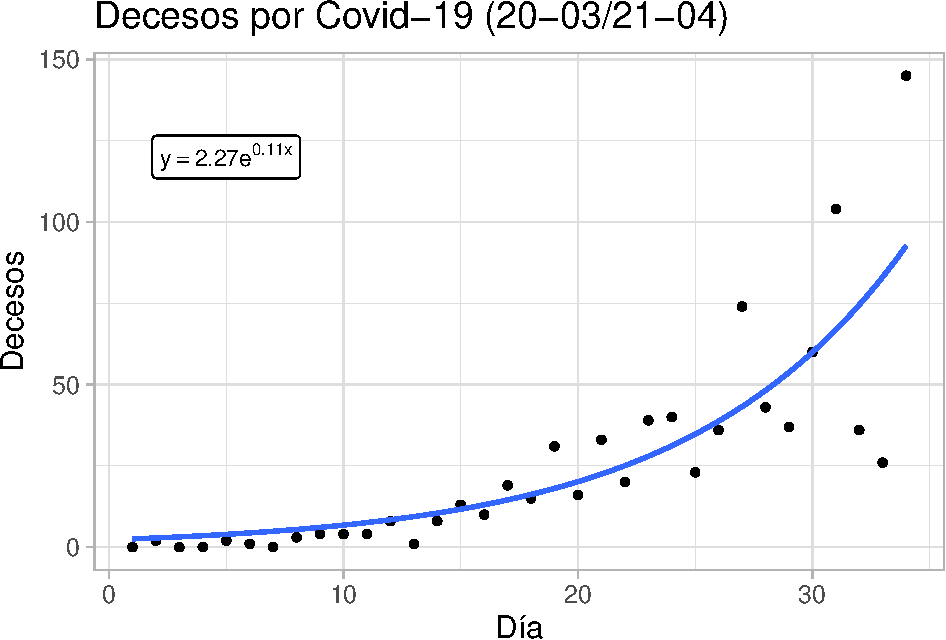
\includegraphics{covid19_mx_files/figure-latex/unnamed-chunk-6-1.pdf}

\begin{Shaded}
\begin{Highlighting}[]
\CommentTok{# La gráfica en PNG del HTML tiene un error de impresión en la fórmula.}
\CommentTok{# Este pedazo de código reemplaza la gráfica de salida del pedazo de código }
\CommentTok{# anterior con una gráfica creada de manera manual, exportada a PDF y}
\CommentTok{# convertida a PNG con inkscape. Esto no ocurre con el formato de salida en PDF.}
\NormalTok{  knitr}\OperatorTok{::}\KeywordTok{include_graphics}\NormalTok{(}\StringTok{'/home/murphy/Repos/plotcovid19mx/Rplot01.png'}\NormalTok{)}
\end{Highlighting}
\end{Shaded}

\end{document}
